% ----------------------------------------------------------
% Capítulo de Resultados
% ----------------------------------------------------------
\chapter{Resultados}
\label{cap:resultados}
% ---

Este capítulo apresenta os resultados da avaliação da plataforma desenvolvida para a Casa de Cultura de João Monlevade, destacando as melhorias na gestão institucional e os impactos positivos que a plataforma trouxe para a automação de processos. Serão discutidos os critérios e métodos de avaliação utilizados, bem como os resultados obtidos em cada um deles.

\section{Critérios de Avaliação}

Os testes e validações da plataforma de artistas monlevadenses foram fundamentados em critérios importantes, que guiaram a avaliação do desempenho geral da plataforma.

\subsection{Funcionalidade} 

O principal objetivo foi verificar se as funcionalidades planejadas, como a publicação de notícias, a exposição dos artistas na "Vitrine", o acompanhamento da Escola de Artes e a divulgação de editais, estavam funcionando corretamente, conforme o escopo do projeto. 

\subsection{Usabilidade} 

Avaliar a facilidade de uso da plataforma foi essencial, levando em consideração a experiência do usuário, a navegabilidade e a acessibilidade. 

\subsection{Desempenho} 

Medimos o tempo de resposta da plataforma sob diferentes cenários de uso, simulando o acesso de um usuário à página principal. A implementação atual do website foi realizada na plataforma PythonAnywhere, utilizando sua categoria gratuita. 

\subsection{Segurança} 
A integridade e proteção dos dados inseridos na plataforma foram rigorosamente avaliadas. O objetivo foi garantir que as informações dos usuários, especialmente dos artistas e administradores, estivessem protegidas contra acessos não autorizados.

\section{Métodos de Avaliação}

Diversos métodos foram aplicados para validar os critérios de avaliação estabelecidos, estes são descritos abaixo.

\subsection{Testes de Funcionalidade} 

Foram realizados testes com um grupo de usuários da Casa de Cultura, incluindo artistas e administradores. Esses testes focaram em validar se a ferramenta atendia corretamente às expectativas em relação às funcionalidades do site. A seção de editais trouxe uma transformação ao integrar um sistema de inscrição online, substituindo o uso anterior de formulários do Google. Essa mudança otimiza a seleção e organização de eventos culturais, proporcionando economia de tempo e recursos aos colaboradores, além de aumentar a transparência, com todas as informações disponíveis de forma clara e acessível.

\subsection{Testes de Usabilidade}

Observou-se a interação dos usuários com as diferentes seções da plataforma, como o formulário de inscrição de artistas e o painel administrativo, com o objetivo de identificar áreas de melhoria na experiência do usuário. A Escola de Artes se beneficiou da informatização dos documentos acadêmicos, permitindo um acompanhamento mais próximo dos alunos. Esse processo facilita o acesso à informação por alunos, professores e responsáveis, otimizando a gestão interna e o fluxo de dados acadêmicos de maneira mais organizada e centralizada.

Durante os testes, foram coletadas impressões dos usuários sobre a navegabilidade e a intuitividade da interface. A maioria dos participantes relatou uma experiência positiva, destacando a clareza nas instruções e a facilidade de localizar as principais funcionalidades. No entanto, algumas sugestões de melhorias foram feitas, como a inclusão de tutoriais visuais para novos usuários e a simplificação de alguns formulários.

Além disso, foi conduzido um teste utilizando a ferramenta automatizada do Google, Page Speed Insights, que graduou o site com notas máximas nos quesitos acessibilidade e uso de práticas recomendadas na categoria de dispositivos móveis, e quase perfeita na categoria Desktop. Esses resultados indicam que o site foi projetado com uma forte ênfase na experiência do usuário, permitindo uma navegação fluida e eficiente em diferentes dispositivos.

\begin{figure}[htb] \caption{\label{fig_grafico}Avaliação Page Speed Insights} \begin{center} 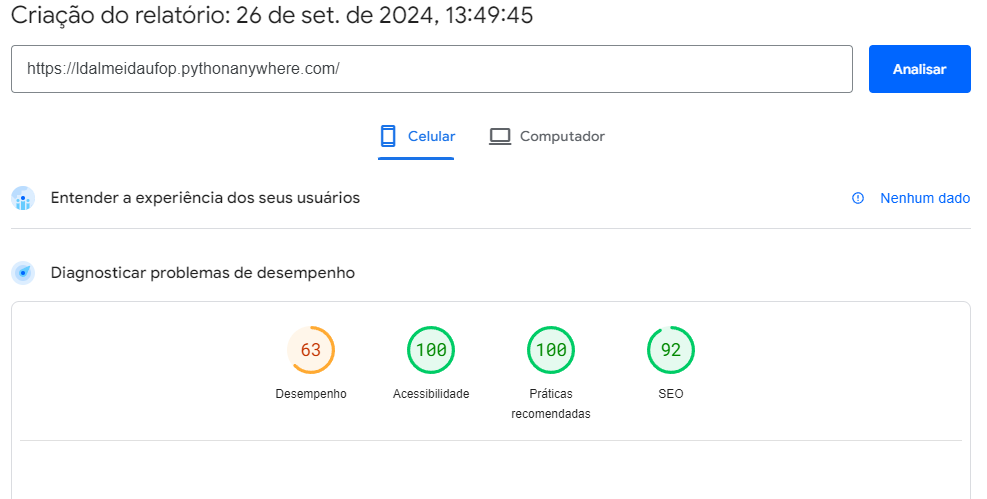
\includegraphics[scale=0.3]{./img/pagespeedinsights.png} \end{center} \legend{Fonte: o autor} \end{figure}

\subsection{Testes de Desempenho}

A escolha de usar um serviço gratuito de hospedagem possibilitou a realização de testes em condições adversas, simulando o pior cenário possível em termos de desempenho, pois os testes foram realizados com a cota de CPU completamente utilizada. Apesar dessas limitações, a plataforma se manteve estável, reforçando seu potencial. Os resultados indicam que, mesmo em condições desfavoráveis, a estrutura da plataforma é robusta e capaz de lidar com a carga de usuários.

Foram utilzadas ferramentas automatizadas de avaliação de sites web. O teste realizado com o GTmetrix retornou uma avaliação de 90\% no quesito performance, demonstrando um bom tempo de resposta para o carregamento da página principal. Essa nota reflete a eficiência do código e a adequação das tecnologias utilizadas na construção do site.

\begin{figure}[htb] \caption{\label{fig_grafico}Avaliação GTmetrix} \begin{center} 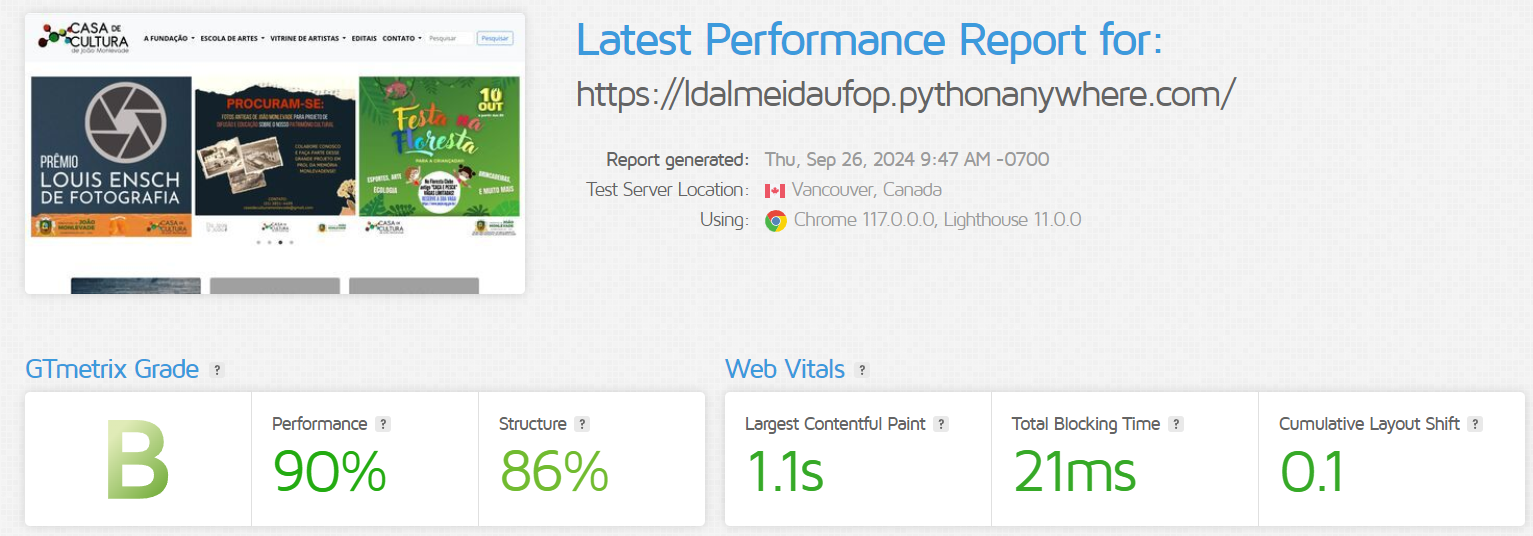
\includegraphics[scale=0.3]{./img/gtmetrix.png} \end{center} \legend{Fonte: o autor} \end{figure}

No entanto, é importante reforçar que esses resultados representam o pior caso. O desempenho da plataforma será consideravelmente melhor quando o site for hospedado pela Prefeitura, que oferecerá mais recursos computacionais e de infraestrutura. Essa migração não só melhorará a velocidade de carregamento, mas também permitirá a implementação de novas funcionalidades que dependem de maior capacidade de processamento.

O código-fonte do site também foi submetido a testes utilizando a ferramenta Validator. A partir dela, detectou-se uma oportunidade de melhoria na organização dos scripts, como pode ser verificado abaixo. Após a refatoração do código, utilizando as boas práticas e reorganizando a importação dos scripts, foi verificada a resolução do problema. Essa etapa de otimização é crucial para garantir a escalabilidade da plataforma, permitindo que ela suporte um aumento no número de usuários sem comprometer o desempenho.

\begin{figure}[htb] \caption{\label{fig_grafico}Erro apontado pelo Validator} \begin{center} 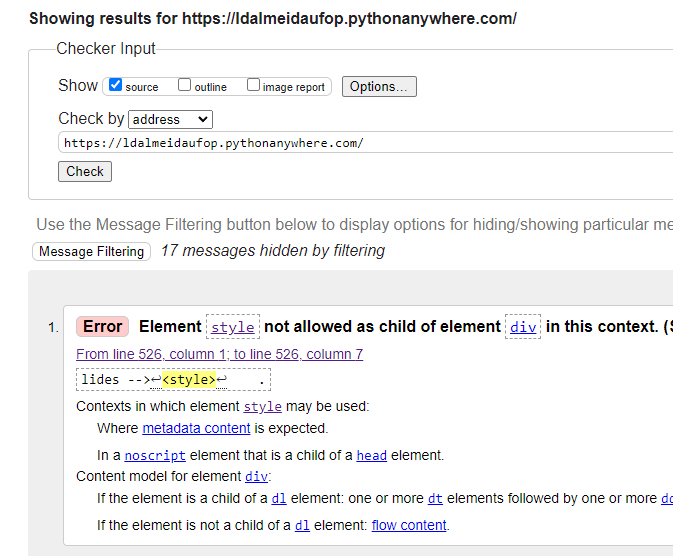
\includegraphics[scale=0.3]{./img/validator_error.png} \end{center} \legend{Fonte: o autor} \end{figure}

\begin{figure}[htb] \caption{\label{fig_grafico}Erro corrigido} \begin{center} 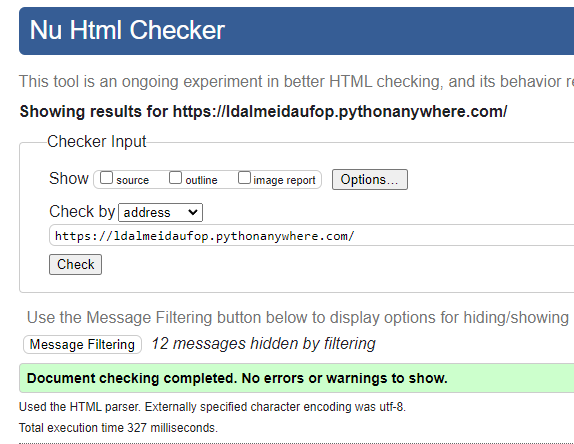
\includegraphics[scale=0.3]{./img/validator_sucess.png} \end{center} \legend{Fonte: o autor} \end{figure}

\subsection{Testes de Segurança}

Os logs gerados por duas plataformas de teste de segurança online foram analizados e ambas não detectaram nenhum risco médio ou grave presente no site, o que demonstra uma preocupação constante com a segurança da informação. O teste realizado pela plataforma Pentest Tools retornou quatro considerações de nível baixo, relacionadas ao certificado de segurança do site, as tecnologias não estarem obfuscadas e o arquivo robots.txt, que instrui \textit{web crawlers} sobre quais \ac{URL} e \textit{endpoints} da aplicação eles podem visitar, estar visível.

\begin{figure}[htb] \caption{\label{fig_grafico}Teste do Pentest Tools} \begin{center} 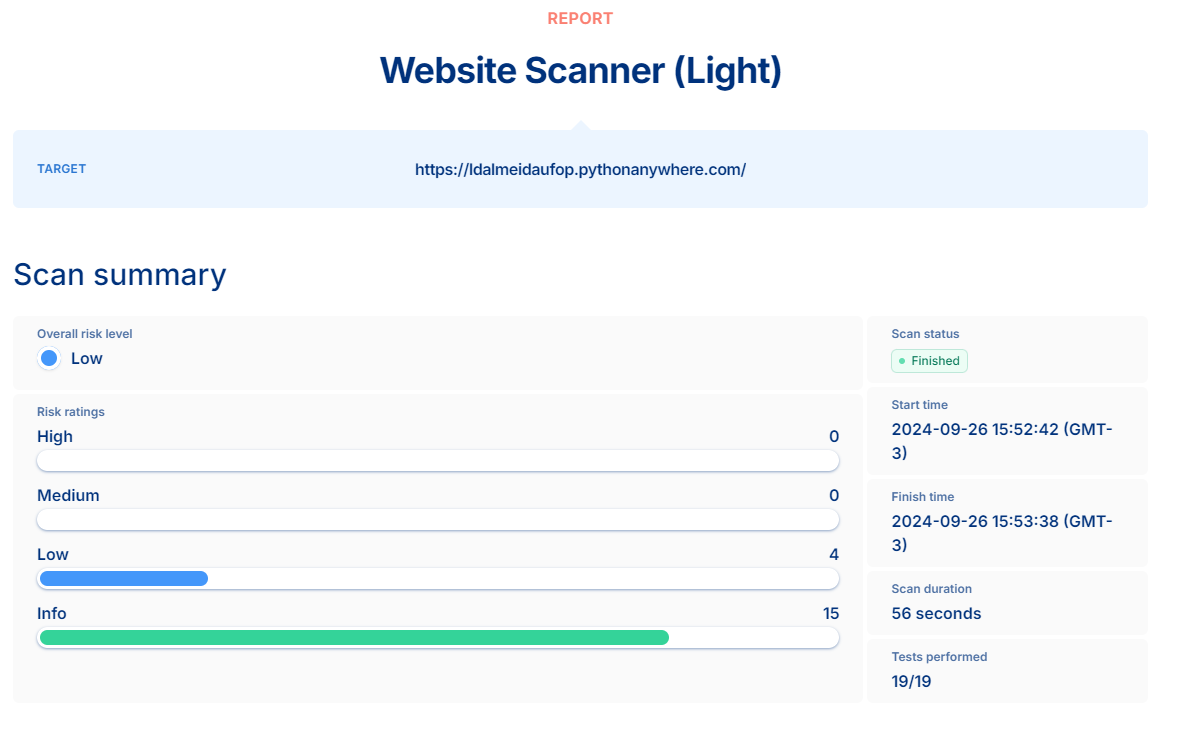
\includegraphics[scale=0.3]{./img/pentest.png} \end{center} \legend{Fonte: o autor} \end{figure}

A outra plataforma utilizada foi a Immuniweb. Os resultados obtidos ao final do teste realizado pela ferramenta graduaram o sistema com a nota "A-". Não foram encontradas vulnerabilidades no sistema; no entanto, foi verificado que dois pacotes estavam desatualizados, mas sem nenhuma vulnerabilidade conhecida. Essa avaliação positiva sugere que a plataforma foi projetada e mantida com um foco significativo em práticas de segurança, o que é crucial para proteger os dados sensíveis dos usuários.

\begin{figure}[htb] \caption{\label{fig_grafico}Teste do Immuniweb} \begin{center} 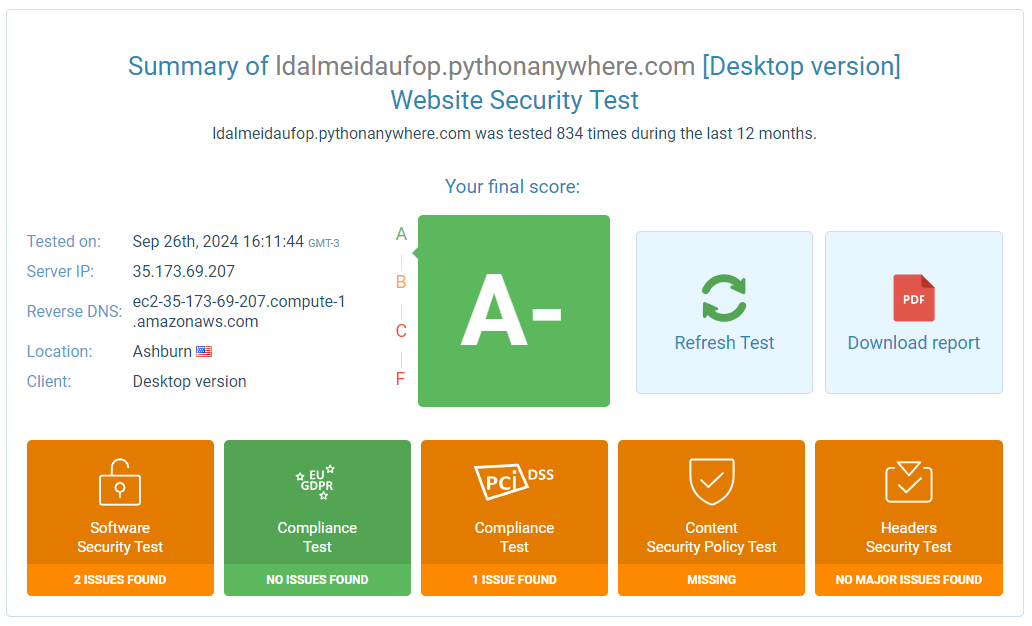
\includegraphics[scale=0.3]{./img/immuniweb.png} \end{center} \legend{Fonte: o autor} \end{figure}

Esses testes de segurança não apenas garantem a integridade da plataforma, mas também reforçam a confiança dos usuários na utilização do sistema. A segurança é um fator crucial, especialmente em plataformas que lidam com dados pessoais e informações acadêmicas, e a adoção de boas práticas de segurança ajudará a manter a credibilidade da Casa de Cultura.

\section{Resultados Obtidos}


Os resultados dos testes indicam que a plataforma atende aos critérios de funcionalidade e usabilidade estabelecidos no início do projeto. As funcionalidades principais operam corretamente, e a interface foi bem avaliada pelos usuários quanto à sua facilidade de uso. Com relação ao desempenho, o sistema mostrou-se robusto, respondendo adequadamente aos testes simulados, sendo necessários apenas pequenos ajustes para otimizar o código-fonte em questões bem pontuais.

Quanto à segurança, os testes não revelaram vulnerabilidades críticas, e as medidas de proteção dos dados se mostraram eficazes. Porém, será necessário que no momento da implantação do site sejam implementadas rotinas de backup automáticas e mecanismos de autenticação robustos ao servidores para garantir a integridade das informações.

Em resumo, a plataforma da Casa de Cultura de João Monlevade se mostrou eficiente nos testes realizados, com bom desempenho, usabilidade adequada e segurança confiável, estando apta a ser utilizada pelos artistas locais e administradores da instituição.